\chapter{Risultati e Discussioni}

In questo capitolo verranno presentati i grafici ottenuti dai \textit{performance test} eseguiti sugli algoritmi in standardizzazione. Ad ogni grafico seguirà una breve argomentazione, se necessaria. Per praticità vengono allegati solo i grafici più significativi, tuttavia nel repository GitHub del progetto \cite{project-github} sono disponibili ulteriori immagini che mettono in relazione aspetti diversi. Il materiale è disponibile nella cartella \textit{plot} del progetto.

La fase di analisi si concentrerà in particolare sulle versioni ottimizzate dei candidati, spesso definite con il termine \textit{AVX2} poiché rappresenta una forma di ottimizzazione comune tra le varie implementazioni. Sono stati prodotti anche grafici che mettono in relazione le caratteristiche delle versioni \textit{REF} e \textit{AVX2}: spesso si rileva un aumento delle prestazioni (in termini di tempi di esecuzione) tra il 50\% e il 100\%.



\section{CRYSTALS Dilithium}

Le versioni di CRYSTALS Dilithium rilasciate per ogni implementazione sono Dilithium 2, Dilithium 3 e Dilithium 5. Come suggerisce il nome, esse sono legate ai livelli di sicurezza offerti, rispettivamente 2, 3 e 5.

Tra queste versioni le principali differenze sono legate ai parametri di generazione della coppia di chiavi e alla generazione della firma. Le dimensioni e tempistiche di ciascuna variante sono riassunte nella tabella \ref{tab:dilithium_comparison}.

In generale, le dimensioni delle chiavi e delle firme sono fisse a parità di versione scelta, questo garantisce una maggior resistenza ai \textit{side channel attacks} e una maggior facilità di standardizzazione.

\begin{figure}[H]
    \centering
    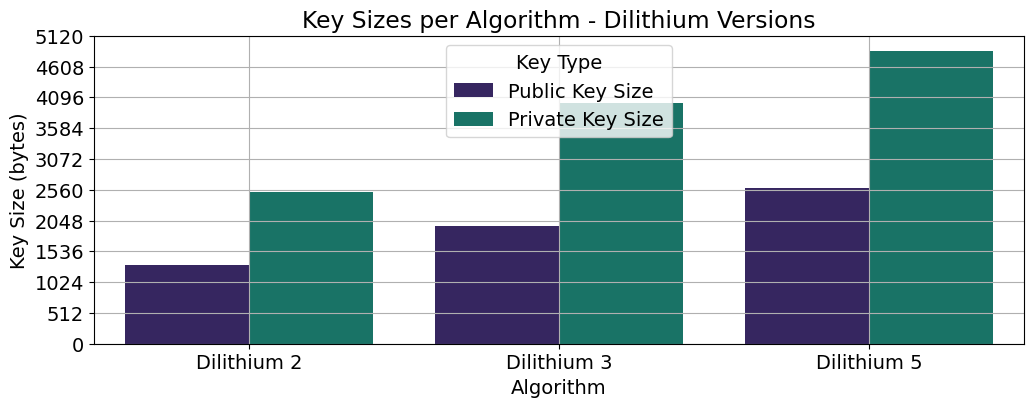
\includegraphics[width=1\textwidth]{Immagini/20240822_i9/Key_Sizes/KC_dilithium.png}
    \caption{Dimensione delle chiavi private e pubbliche per le versioni di CRYSTALS Dilithium}
    \label{fig:KC_dilithium}
\end{figure}

Il grafico \ref{fig:KC_dilithium} evidenzia la differenza di dimensioni tra le chiavi pubbliche e le chiavi private. Inoltre, ogni gruppo di colonne rappresenta una delle versioni di Dilithium: si evince che la dimensione delle chiavi cresce con andamento lineare al livello di sicurezza offerto.

\begin{figure}[H]
    \centering
    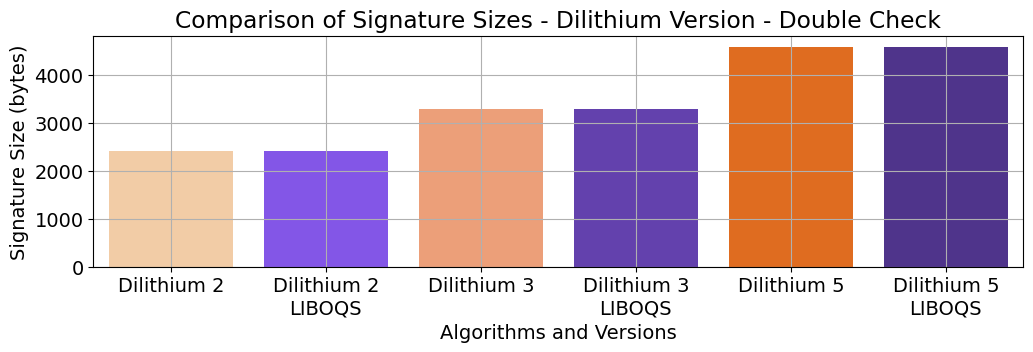
\includegraphics[width=1\textwidth]{Immagini/20240822_i9/Message_IO/double_check/IO_dilithium.png}
    \caption{Confronto delle dimensioni delle firme tra l'implementazione diretta e l'implementazione LibOQS per CRYSTALS Dilithium}
    \label{fig:IO_dilithium}
\end{figure}

Il grafico \ref{fig:IO_dilithium} mostra uno dei test di verifica tra l'implementazione diretta e l'implementazione tramite libreria \textit{LibOQS}. Si può notare come i dati coincidano per ogni versione inoltre, come per le chiavi anche la dimensione della firma sembra aumentare in dimensione con andamento lineare al livello di sicurezza.

\begin{figure}[H]
    \centering
    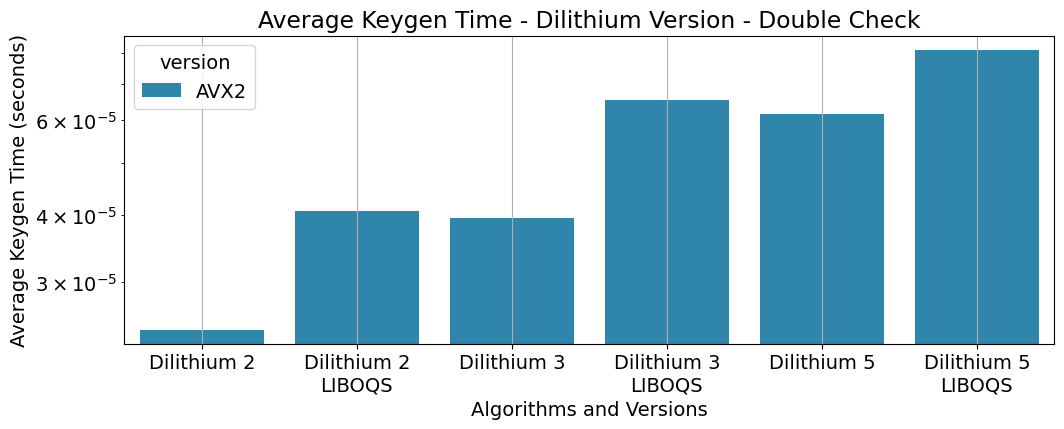
\includegraphics[width=1\textwidth]{Immagini/20240822_i9/Time_Keygen/double_check/TM_KG_dilithium.png}
    \caption{Confronto dei tempi di generazione chiavi tra l'implementazione diretta e l'implementazione LibOQS per CRYSTALS Dilithium}
    \label{fig:TM_KG_dilithium}
\end{figure}

I tempi di \textit{keygen} nel grafico \ref{fig:TM_KG_dilithium} mostrano una maggior rapidità di esecuzione nell'implementazione diretta. Probabilmente questo accade perché la libreria \textit{LibOQS} è un \textit{wrapper} degli algoritmi originali, dunque come tale aggiunge dell'\textit{overhead}. In ogni caso, le tempistiche si trovano sullo stesso ordine di grandezza, dunque le differenze non sono significative.

\begin{figure}[H]
    \centering
    \begin{minipage}{0.45\textwidth}
        \centering
        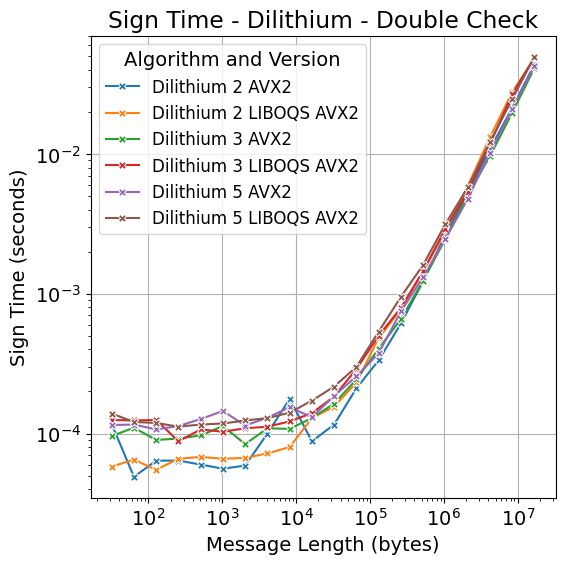
\includegraphics[width=1\textwidth]{Immagini/20240822_i9/Time_Sign/double_check/TM_SG_dilithium.png}
        \caption{Controllo dei tempi di firma con LibOQS per CRYSTALS Dilithium con messaggi di lunghezza variabile}
        \label{fig:TM_SG_dilithium}
    \end{minipage}\hfill
    \begin{minipage}{0.45\textwidth}
        \centering
        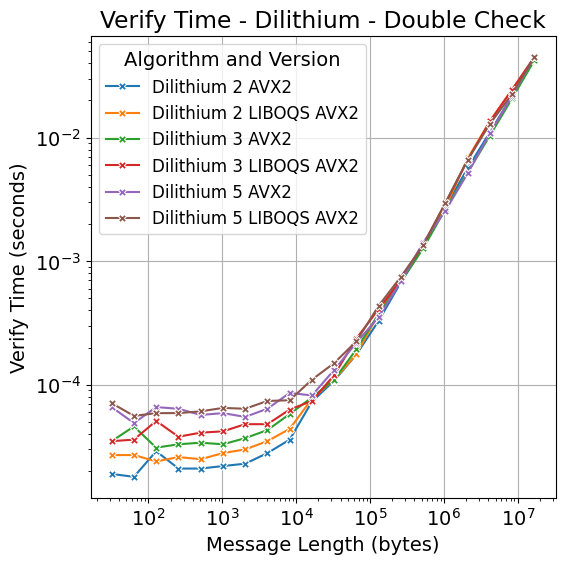
\includegraphics[width=1\textwidth]{Immagini/20240822_i9/Time_Verify/double_check/TM_VF_dilithium.png}
        \caption{Controllo dei tempi di verifica con LibOQS per CRYSTALS Dilithium con messaggi di lunghezza variabile}
        \label{fig:TM_VF_dilithium}
    \end{minipage}
\end{figure}

Il grafico \ref{fig:TM_SG_dilithium} e \ref{fig:TM_VF_dilithium} evidenziano come CRYSTALS Dilithium comporti un aumento dei tempi esponenziale (l'asse dei tempi ha scala logaritmica) quando la dimensione del messaggio da firmare o verificare cresce oltre l'ordine dei KiloBytes.

In ogni caso, utilizzando operazioni piuttosto efficienti (tra vettori e matrici) i tempi rimangono comunque ridotti anche in caso di messaggi nell'ordine dei MegaBytes.

\begin{figure}[H]
    \centering
    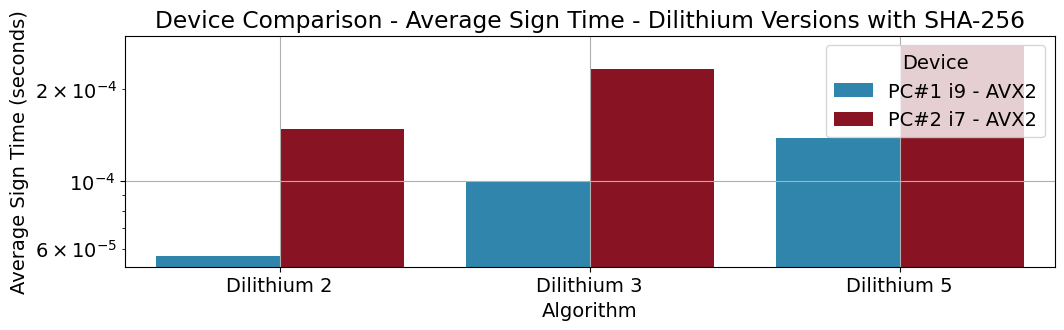
\includegraphics[width=1\textwidth]{Immagini/comparison/Time_Sign/TM_SG_H_dilithium_sha256.png}
    \caption{Tempi di firma con messaggi di lunghezza fissa su PC\#1 e PC\#2 per CRYSTALS Dilithium}
    \label{fig:TM_SG_H_dilithium_sha256}
\end{figure}

Il grafico \ref{fig:TM_SG_H_dilithium_sha256} è più significativo del precedente per i tempi di firma poiché considera il comune scenario in cui il messaggio subisce un processo di \textit{hashing} prima della creazione della firma. In questo caso l'\textit{hashing} è stato effettuato con i sistemi attualmente più utilizzati, cioè \textit{SHA-256} e \textit{SHA-512}. Con entrambe queste tecniche i tempi di firma hanno esecuzioni più rapide sui dispositivi utilizzati per la fase di test. In entrambi i dispositivi di test i tempi di firma sono direttamente proporzionali al livello di sicurezza offerto dall'algoritmo utilizzato: algoritmi più sicuri implicano tempi di esecuzione maggiori.

\begin{figure}[H]
    \centering
    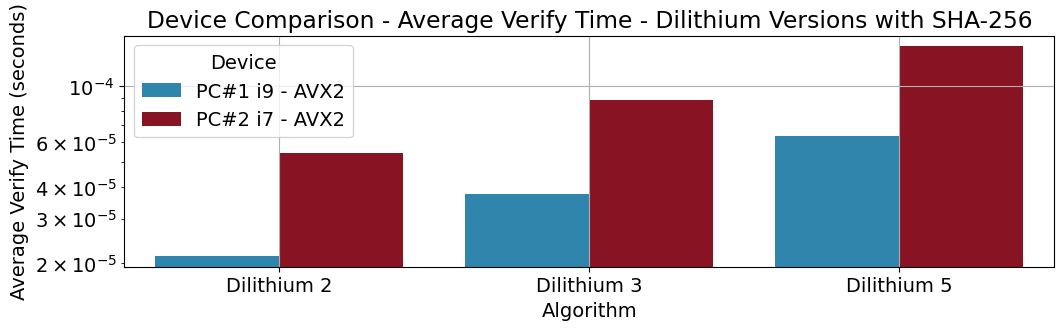
\includegraphics[width=1\textwidth]{Immagini/comparison/Time_Verify/TM_VF_H_dilithium_sha256.png}
    \caption{Tempi di verifica con messaggi di lunghezza fissa su PC\#1 e PC\#2 per CRYSTALS Dilithium}
    \label{fig:TM_VF_H_dilithium_sha256}
\end{figure}

Allo stesso modo il grafico \ref{fig:TM_VF_H_dilithium_sha256} è significativo per i tempi di verifica della firma. Le funzioni di \textit{hashing} utilizzate sono le medesime cioè \textit{SHA-256} e \textit{SHA-512}. In generale si può notare come in entrambi i dispositivi le operazioni di verifica richiedano inferiore tempo rispetto alla firma. Quest'ultima è una caratteristica che accomuna la maggior parte dei sistemi di firma digitale. È intrinseca nel loro metodo di funzionamento poiché la verifica di un messaggio richiede operazioni di minor complessità.

Successivamente viene proposta una tabella (\ref{tab:dilithium_comparison}) riassuntiva con le medie dei tempi e le occupazioni in memoria di chiavi e firme. Quest'ultima mette in relazione le versioni \textit{AVX2} e \textit{REF} di cui non vengono presentati i grafici.

\begin{table}[H]
    \centering
    \begin{tabular}{lccc}
        \toprule
        & \textbf{Dilithium 2} & \textbf{Dilithium 3} & \textbf{Dilithium 5} \\
        \cmidrule(lr){1-4}
        \textbf{Dimensione chiave privata (bytes)} & 2528 & 4000 & 4864 \\
        \textbf{Dimensione chiave pubblica (bytes)} & 1312 & 1952 & 2592 \\
        \textbf{Dimensione firma (bytes)} & 2420 & 3293 & 4595 \\
        \textbf{Livello di sicurezza (bytes)} & 2 & 3 & 5 \\
        \midrule
        \multicolumn{4}{c}{\textbf{REF}} \\
        \cmidrule(lr){1-4}
        \textbf{Tempo medio Key Gen (ns)} & 68 & 118 & 174 \\
        \textbf{Tempo medio firma SHA256 (ns)} & 277 & 431 & 567 \\
        \textbf{Tempo medio firma SHA512 (ns)} & 254 & 430 & 519 \\
        \textbf{Tempo medio verifica SHA256 (ns)} & 72 & 117 & 180 \\
        \textbf{Tempo medio verifica SHA512 (ns)} & 71 & 113 & 169 \\
        \midrule
        \multicolumn{4}{c}{\textbf{AVX2}} \\
        \cmidrule(lr){1-4}
        \textbf{Tempo medio Key Gen (ns)} & 23 & 46 & 66 \\
        \textbf{Tempo medio firma SHA256 (ns)} & 52 & 105 & 138 \\
        \textbf{Tempo medio firma SHA512 (ns)} & 56 & 113 & 146 \\
        \textbf{Tempo medio verifica SHA256 (ns)} & 20 & 36 & 61 \\
        \textbf{Tempo medio verifica SHA512 (ns)} & 20 & 40 & 67 \\
        \bottomrule
    \end{tabular}
    \caption{Confronto tra versioni \textit{REF} e \textit{AVX2} di CRYSTALS Dilithium. Tempi riferiti all'esecuzione su PC\#1}
    \label{tab:dilithium_comparison}
\end{table}



\section{FALCON}

Per ogni implementazione, sia essa ottimizzata o di riferimento, le versioni disponibili sono \textit{FALCON 512} e \textit{FALCON 1024}, i cui livelli di sicurezza sono rispettivamente 1 e 5. Questo candidato alla standardizzazione offre un inferiore numero di livelli di sicurezza disponibili, tuttavia essi sono i valori agli estremi della scala.

\begin{figure}[H]
    \centering
    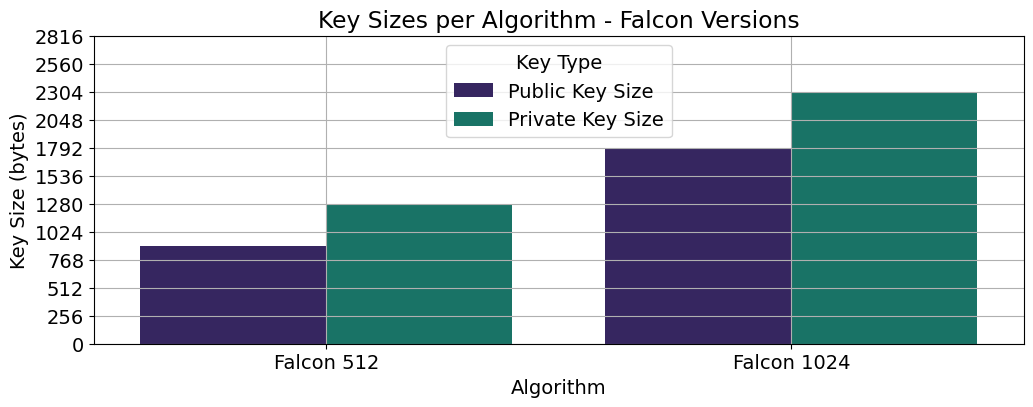
\includegraphics[width=1\textwidth]{Immagini/20240822_i9/Key_Sizes/KC_falcon.png}
    \caption{Dimensione delle chiavi private e pubbliche per le versioni di FALCON}
    \label{fig:KC_falcon}
\end{figure}

Nonostante ciò, dal grafico \ref{fig:KC_falcon} è possibile notare come la differenza in dimensioni tra le chiavi non sia eccessiva. Al contrario, proprio perché uno degli obiettivi secondari di FALCON era la compattezza, le sue chiavi sono tra le più corte se prendiamo in considerazione solo i sistemi di firma digitale \textit{Lattice Based}.

\begin{figure}[H]
    \centering
    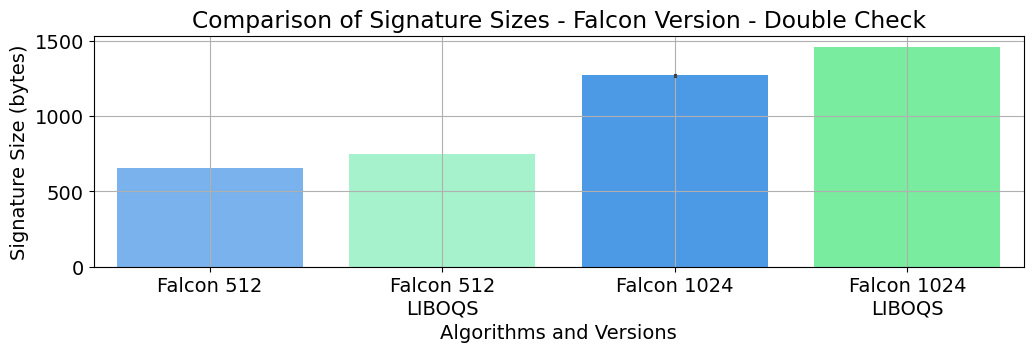
\includegraphics[width=1\textwidth]{Immagini/20240822_i9/Message_IO/double_check/IO_falcon.png}
    \caption{Confronto delle dimensioni delle firme tra l'implementazione diretta e l'implementazione LibOQS per FALCON}
    \label{fig:IO_falcon}
\end{figure}

Le stesse caratteristiche si notano nel grafico \ref{fig:IO_falcon}: la dimensione della firma è piuttosto limitata. Si nota un altro aspetto importante: al contrario di CRYSTALS Dilithium, la dimensione della firma tra l'implementazione diretta e l'implementazione tramite libreria \textit{LibOQS} differisce. Ciò accade perché l'implementazione diretta utilizza una versione di FALCON che genera la firma più compatta possibile, rendendo la dimensione delle firme non costante. Invece la libreria \textit{LibOQS} implementa una versione di FALCON con \textit{zero-padding} sulla firma, così da rendere l'uso del sistema di firma più uniforme e più resistente ai \textit{side channel attacks}.

\begin{figure}[H]
    \centering
    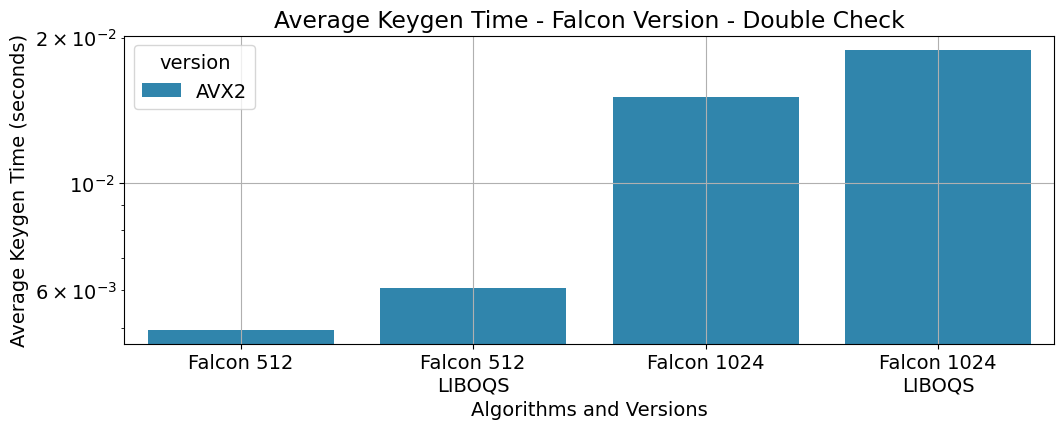
\includegraphics[width=1\textwidth]{Immagini/20240822_i9/Time_Keygen/double_check/TM_KG_falcon.png}
    \caption{Confronto dei tempi di generazione chiavi tra l'implementazione diretta e l'implementazione LibOQS per FALCON}
    \label{fig:TM_KG_falcon}
\end{figure}

I tempi di \textit{keygen} nel grafico \ref{fig:TM_KG_falcon} rispecchiano maggiormente la differenza di livelli di sicurezza offerti dalle due varianti di FALCON. Ancora una volta \textit{LibOQS} risulta leggermente più lenta, probabilmente per operazioni aggiuntive dovute al \textit{wrapping}.

\begin{figure}[H]
    \centering
    \begin{minipage}{0.45\textwidth}
        \centering
        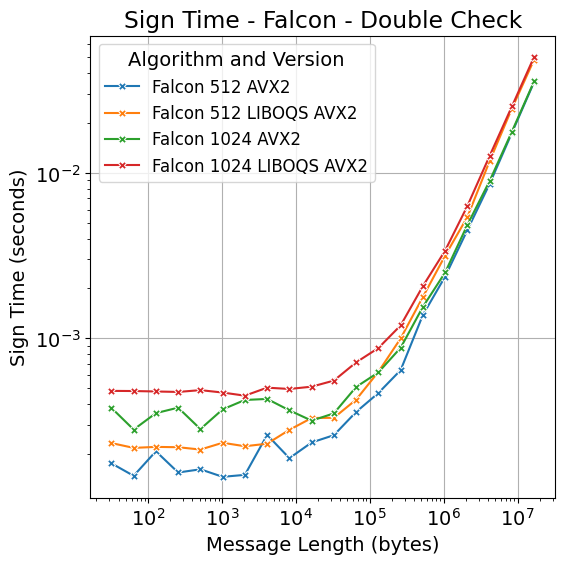
\includegraphics[width=1\textwidth]{Immagini/20240822_i9/Time_Sign/double_check/TM_SG_falcon.png}
        \caption{Controllo dei tempi di firma con LibOQS per FALCON con messaggi di lunghezza variabile}
        \label{fig:TM_SG_falcon}
    \end{minipage}\hfill
    \begin{minipage}{0.45\textwidth}
        \centering
        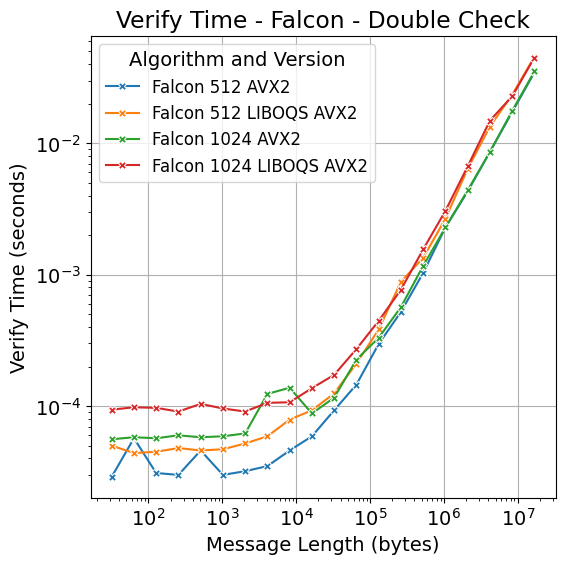
\includegraphics[width=1\textwidth]{Immagini/20240822_i9/Time_Verify/double_check/TM_VF_falcon.png}
        \caption{Controllo dei tempi di verifica con LibOQS per FALCON con messaggi di lunghezza variabile}
        \label{fig:TM_VF_falcon}
    \end{minipage}
\end{figure}

Anche FALCON, come Dilithium, presenta nei grafici \ref{fig:TM_SG_falcon} e \ref{fig:TM_VF_falcon} un aumento dei tempi esponenziale quando la dimensione del messaggio da firmare e verificare cresce oltre l'ordine dei KiloBytes.

\begin{figure}[H]
    \centering
    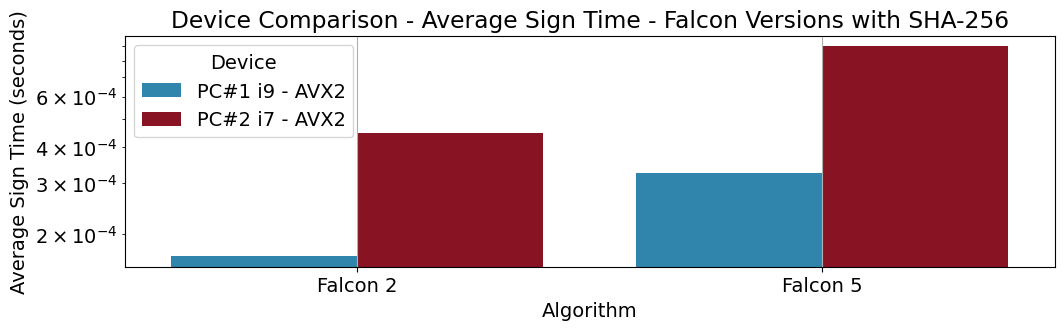
\includegraphics[width=1\textwidth]{Immagini/comparison/Time_Sign/TM_SG_H_falcon_sha256.png}
    \caption{Tempi di firma con messaggi di lunghezza fissa su PC\#1 e PC\#2 per FALCON}
    \label{fig:TM_SG_H_falcon_sha256}
\end{figure}

Per quanto riguarda i test che includono l'\textit{hashing} del messaggio, il grafico \ref{fig:TM_SG_H_falcon_sha256} mostra che i tempi di firma rimangono ridotti su i dispositivi utilizzati per la fase di test, permettendo di effettuare circa un migliaio di operazioni di firma al secondo, come evidenziato anche dal team di ricerca nella relativa documentazione \cite{falcon-submissionpackage-three}.

\begin{figure}[H]
    \centering
    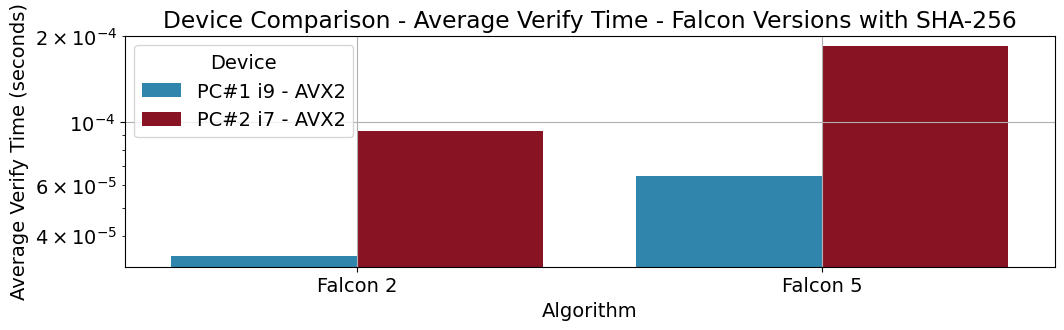
\includegraphics[width=1\textwidth]{Immagini/comparison/Time_Verify/TM_VF_H_falcon_sha256.png}
    \caption{Tempi di verifica con messaggi di lunghezza fissa su PC\#1 e PC\#2 per FALCON}
    \label{fig:TM_VF_H_falcon_sha256}
\end{figure}

Allo stesso modo, nel grafico \ref{fig:TM_VF_H_falcon_sha256}, i tempi di verifica con \textit{hashing} del messaggio mostrano un incremento delle performance di circa un ordine di grandezza rispetto ai tempi di firma.

La differenza tra i risultati di performance dei due dispositivi è piuttosto lineare. Con tutta probabilità tale differenza è dovuta al salto prestazionale tra i due processori (frequenza base, numero di cores, eccetera) piuttosto che a peculiarità dell'algoritmo in esecuzione.

Successivamente vengono riassunte le informazioni nella tabella \ref{tab:falcon_comparison}. Quest'ultima mette in relazione le versioni \textit{AVX2} e \textit{REF}, di cui non sono stati presentati i grafici.

\begin{table}[H]
    \centering
    \begin{tabular}{lcc}
        \toprule
        & \textbf{FALCON 512} & \textbf{FALCON 1024} \\
        \cmidrule(lr){1-3}
        \textbf{Dimensione chiave privata (bytes)} & 1281 & 2305 \\
        \textbf{Dimensione chiave pubblica (bytes)} & 897 & 1793 \\
        \textbf{Dimensione firma (bytes)} & 752 & 1462 \\
        \textbf{Livello di sicurezza (bytes)} & 1 & 5 \\
        \midrule
        \multicolumn{3}{c}{\textbf{REF}} \\
        \cmidrule(lr){1-3}
        \textbf{Tempo medio Key Gen (ns)} & 4986 & 14667 \\
        \textbf{Tempo medio firma SHA256 (ns)} & 201 & 426 \\
        \textbf{Tempo medio firma SHA512 (ns)} & 211 & 390 \\
        \textbf{Tempo medio verifica SHA256 (ns)} & 32 & 60 \\
        \textbf{Tempo medio verifica SHA512 (ns)} & 34 & 59 \\
        \midrule
        \multicolumn{3}{c}{\textbf{AVX2}} \\
        \cmidrule(lr){1-3}
        \textbf{Tempo medio Key Gen (ns)} & 5032 & 14965 \\
        \textbf{Tempo medio firma SHA256 (ns)} & 168 & 330 \\
        \textbf{Tempo medio firma SHA512 (ns)} & 184 & 308 \\
        \textbf{Tempo medio verifica SHA256 (ns)} & 32 & 59 \\
        \textbf{Tempo medio verifica SHA512 (ns)} & 33 & 58 \\
        \bottomrule
    \end{tabular}
    \caption{Confronto tra le versioni \textit{REF} e \textit{AVX2} di FALCON. Tempi riferiti all'esecuzione su PC\#1}
    \label{tab:falcon_comparison}
\end{table}



\section{SPHINCS+}

Come anticipato nei capitoli precedenti, le implementazioni di SPHINCS+ si diversificano per la funzione di \textit{hashing} utilizzata. poiché l'implementazione \textit{Haraka} attualmente risulta poco sicura, tra le soluzioni \textit{SHA256} e \textit{SHAKE256} è stata selezionata la prima.

Sulla base di questa, sono poi state considerate le rispettive versioni \textit{REF} e \textit{AVX2} in tutte le varianti richieste dai test, cioè SPHINCS+ 128, SPHINCS+ 192 e SPHINCS+ 256 che offrono rispettivamente i livelli di sicurezza 2, 3 e 5, come CRYSTALS Dilithium.

\begin{figure}[H]
    \centering
    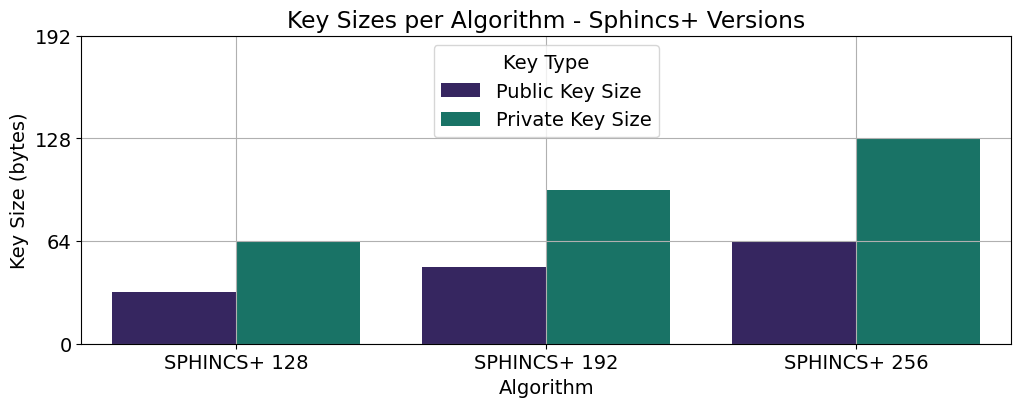
\includegraphics[width=1\textwidth]{Immagini/20240822_i9/Key_Sizes/KC_sphincs.png}
    \caption{Dimensione delle chiavi private e pubbliche per le versioni di SPHINCS+}
    \label{fig:KC_sphincs}
\end{figure}

Il grafico \ref{fig:KC_sphincs} mette subito in evidenza una caratteristica fondamentale di SPHINCS+: le chiavi hanno dimensioni ridottissime, pari a qualche decina di bytes. Questo perché SPHINCS+ è un sistema di firma digitale \textit{Hash Based}.

\begin{figure}[H]
    \centering
    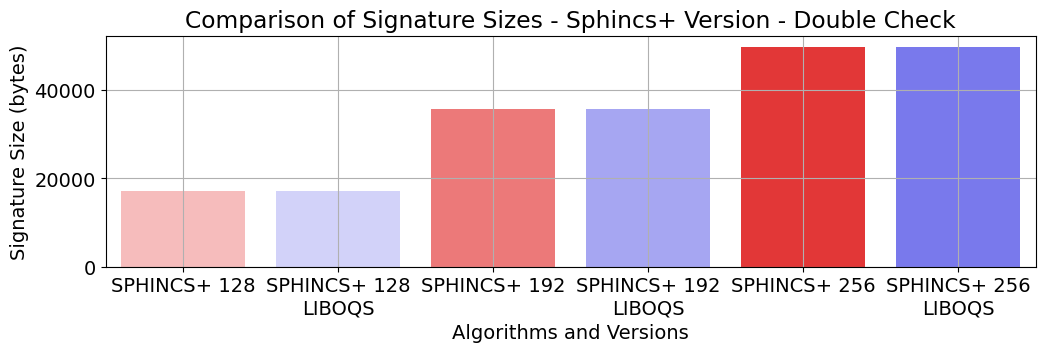
\includegraphics[width=1\textwidth]{Immagini/20240822_i9/Message_IO/double_check/IO_sphincs.png}
    \caption{Confronto delle dimensioni delle firme tra l'implementazione diretta e l'implementazione LibOQS per SPHINCS+}
    \label{fig:IO_sphincs}
\end{figure}

Al contrario, le dimensioni delle firme sono molto elevate, come è possibile notare dal grafico \ref{fig:IO_sphincs}. La dimensione delle firme è costante per ciascuna versione dell'algoritmo, dunque sia l'implementazione diretta che l'implementazione con \textit{LibOQS} hanno riportato gli stessi risultati.

\begin{figure}[H]
    \centering
    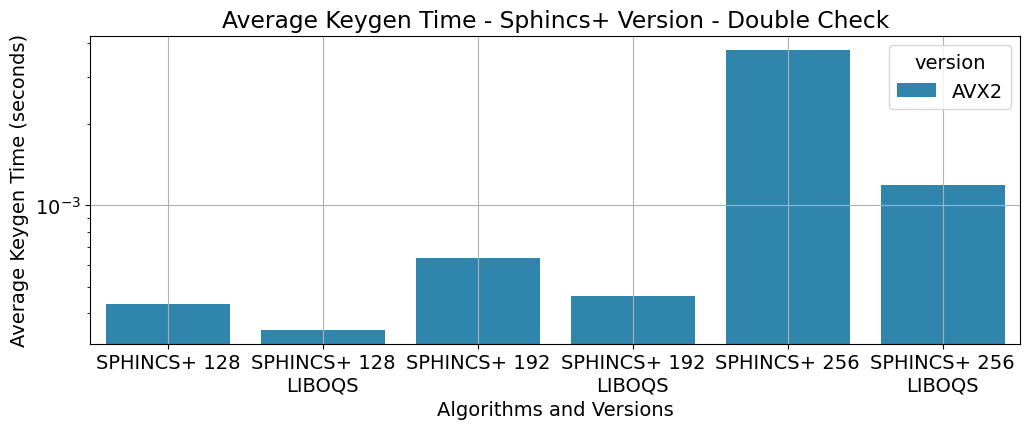
\includegraphics[width=1\textwidth]{Immagini/20240822_i9/Time_Keygen/double_check/TM_KG_sphincs.png}
    \caption{Confronto dei tempi di generazione chiavi tra l'implementazione diretta e l'implementazione LibOQS per SPHINCS+}
    \label{fig:TM_KG_sphincs}
\end{figure}

I tempi di \textit{keygen} nel grafico \ref{fig:TM_KG_sphincs} rispecchiano la differenza di livello di sicurezza offerta dalle versioni di SPHINCS+ in maniera analoga a quanto visto per i precedenti candidati.

In questo caso l'implementazione della libreria \textit{LibOQS} risulta la più veloce in tutti gli ambiti (sia per la generazione delle chiavi, sia in firma e verifica). Questa peculiarità è probabilmente dovuta ai parametri di compilazione di SPHINCS+ introdotti da \textit{LibOQS}, tali da aumentare il numero di ottimizzazioni rispetto all'implementazione diretta offerta. In ogni caso i risultati rimangono sullo stesso ordine di grandezza, per cui possono essere considerati validi.

\begin{figure}[H]
    \centering
    \begin{minipage}{0.45\textwidth}
        \centering
        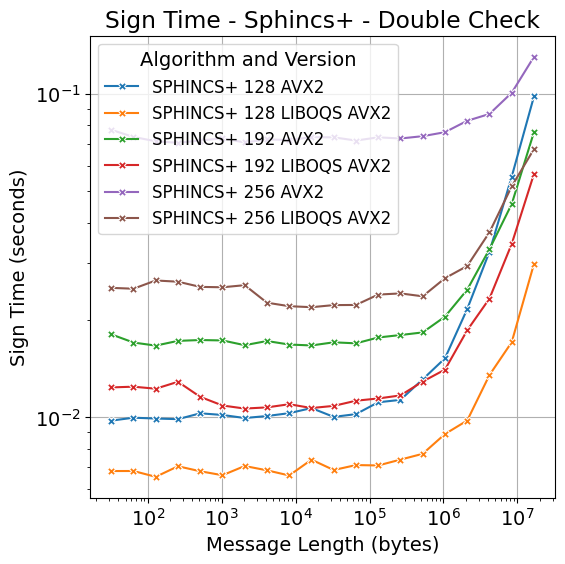
\includegraphics[width=1\textwidth]{Immagini/20240822_i9/Time_Sign/double_check/TM_SG_sphincs.png}
        \caption{Controllo dei tempi di firma con LibOQS per SPHINCS+ con messaggi di lunghezza variabile}
        \label{fig:TM_SG_sphincs}
    \end{minipage}\hfill
    \begin{minipage}{0.45\textwidth}
        \centering
        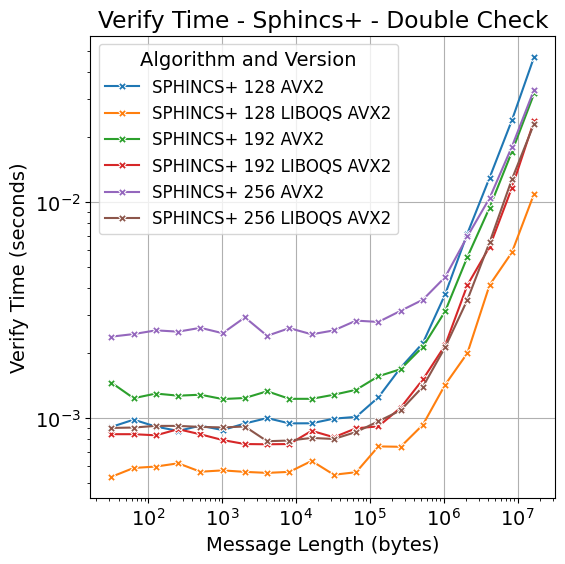
\includegraphics[width=1\textwidth]{Immagini/20240822_i9/Time_Verify/double_check/TM_VF_sphincs.png}
        \caption{Controllo dei tempi di verifica con LibOQS per SPHINCS+ con messaggi di lunghezza variabile}
        \label{fig:TM_VF_sphincs}
    \end{minipage}
\end{figure}

I grafici \ref{fig:TM_SG_sphincs} e \ref{fig:TM_VF_sphincs} rivelano un comportamento unico di SPHINCS+, dovuto alla natura degli algoritmi \textit{Hash Based}. L'aumento esponenziale dei tempi di firma e verifica viene assunto quando il messaggio (elaborato senza tecniche di \textit{hashing}) raggiunge dimensioni nell'ordine dei MegaBytes. Prima di tale soglia i tempi si mantengono piuttosto costanti e, in generale, sono molto più elevati rispetto agli altri candidati.

Questi aspetti sono dovuti all'alta presenza di operazioni di \textit{hashing} all'interno degli algoritmi di SPHINCS+: essi \textit{appiattiscono} le differenze di tempi dovute alla dimensione dell'input e rallentano i tempi di esecuzione poiché sono operazioni onerose.

\begin{figure}[H]
    \centering
    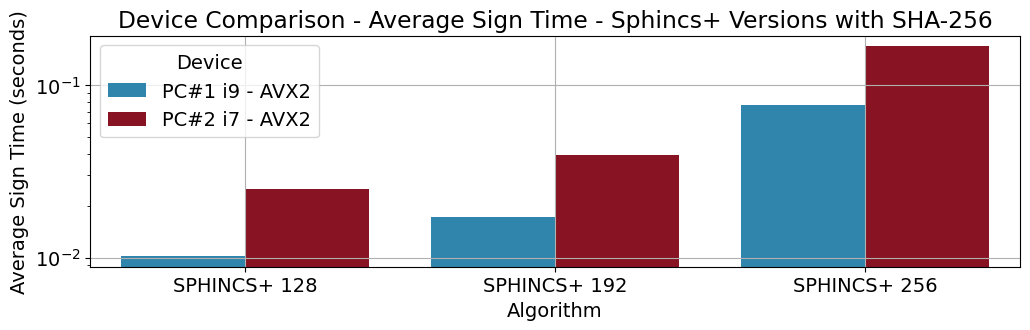
\includegraphics[width=1\textwidth]{Immagini/comparison/Time_Sign/TM_SG_H_sphincs_sha256.png}
    \caption{Tempi di firma con messaggi di lunghezza fissa su PC\#1 e PC\#2 per SPHINCS+}
    \label{fig:TM_SG_H_sphincs_sha256}
\end{figure}

\begin{figure}[H]
    \centering
    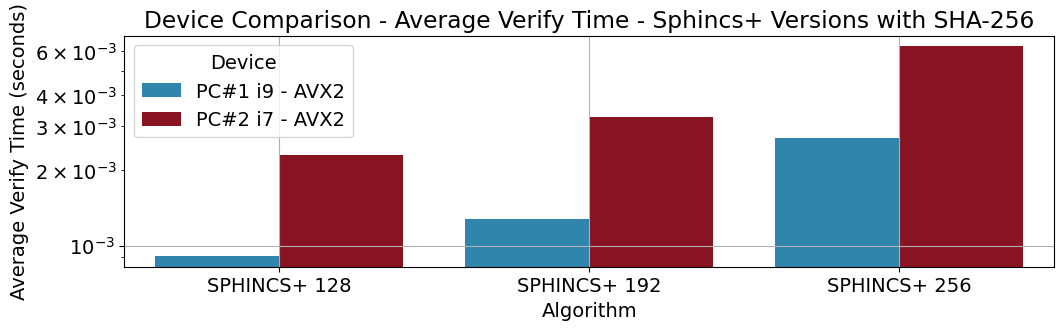
\includegraphics[width=1\textwidth]{Immagini/comparison/Time_Verify/TM_VF_H_sphincs_sha256.png}
    \caption{Tempi di verifica con messaggi di lunghezza fissa su PC\#1 e PC\#2 per SPHINCS+}
    \label{fig:TM_VF_H_sphincs_sha256}
\end{figure}

I test che includono l'\textit{hashing} del messaggio con \textit{SHA-256} e \textit{SHA-512}, evidenziati nei grafici \ref{fig:TM_SG_H_sphincs_sha256} e \ref{fig:TM_VF_H_sphincs_sha256}, mostrano tempistiche che difficilmente permettono di effettuare numeri elevati di firme e verifiche al secondo. Le tempistiche aumentano in maniera esponenziale al livello di sicurezza offerto.

Di seguito è presente un riassunto in formato tabellare dei dati precedenti. La tabella \ref{tab:sphincs_comparison} mette in relazione le versioni \textit{AVX2} e \textit{REF} di SPHINCS+, di cui non sono stati presentati i grafici.

\begin{table}[H]
    \centering
    \begin{tabular}{lccc}
        \toprule
        \textbf{SPHINCS+ Versione:} & \textbf{S+ 128} & \textbf{S+ 192} & \textbf{S+ 256} \\
        \cmidrule(lr){1-4}
        \textbf{Dimensione chiave privata (bytes)} & 64 & 96 & 128 \\
        \textbf{Dimensione chiave pubblica (bytes)} & 32 & 48 & 64 \\
        \textbf{Dimensione firma (bytes)} & 17088 & 16224 & 29792 \\
        \textbf{Livello di sicurezza} & 2 & 3 & 5 \\
        \midrule
        \multicolumn{4}{c}{\textbf{REF}} \\
        \cmidrule(lr){1-4}
        \textbf{Tempo medio Key Gen (ns)} & 1961 & 2967 & 10366 \\
        \textbf{Tempo medio firma SHA256 (ns)} & 46825 & 75216 & 202425 \\
        \textbf{Tempo medio firma SHA512 (ns)} & 46302 & 76296 & 199154 \\
        \textbf{Tempo medio verifica SHA256 (ns)} & 2861 & 4310 & 5883 \\
        \textbf{Tempo medio verifica SHA512 (ns)} & 2888 & 4382 & 5786 \\
        \midrule
        \multicolumn{4}{c}{\textbf{AVX2}} \\
        \cmidrule(lr){1-4}
        \textbf{Tempo medio Key Gen (ns)} & 437 & 644 & 3955 \\
        \textbf{Tempo medio firma SHA256 (ns)} & 10105 & 17201 & 76303 \\
        \textbf{Tempo medio firma SHA512 (ns)} & 10119 & 17284 & 74597 \\
        \textbf{Tempo medio verifica SHA256 (ns)} & 921 & 1272 & 2714 \\
        \textbf{Tempo medio verifica SHA512 (ns)} & 897 & 1280 & 2688 \\
        \bottomrule
    \end{tabular}
    \caption{Confronto tra versioni \textit{REF} e \textit{AVX2} di SPHINCS+. Tempi riferiti all'esecuzione su PC\#1}
    \label{tab:sphincs_comparison}
\end{table}


\section{RSA}

Per poter comprendere meglio la bontà delle prestazioni degli algoritmi PQC, sono stati eseguiti dei test simili anche su una delle tecniche attualmente utilizzate nei processi di firma digitale, ovvero RSA.

Sono state considerate tutte le versioni di RSA associate ai vari livelli di sicurezza. Nella tabella riassuntiva finale è stata aggiunta una riga per specificare i vari \textit{Modulus} di ciascuna versione, cioè la stringa da cui vengono generate le chiavi private e pubbliche. 

Solitamente le versioni di RSA non vengono riconosciute in funzione del livello di sicurezza o della dimensione delle chiavi, bensì in funzione del \textit{Modulus}, dunque quando si parla di RSA 1024 si sta identificando l'algoritmo RSA che utilizza chiavi generate a partire da un \textit{Modulus} di 1024 bits.

L'inclusione delle versioni meno sicure di RSA nei test è motivata dal loro grande utilizzo, dunque gli obiettivi dei nuovi algoritmi PQC in termini di performance dovrebbero essere tarati proprio sui risultati di queste versioni di RSA, sebbene poco sicure.

I test su RSA sono stati implementati utilizzando direttamente le librerie \textit{OpenSSL} installate nel sistema operativo, dunque a differenza degli altri algoritmi non è stato utilizzato e compilato alcun codice sorgente, escluso quello di implementazione dei \textit{performance test}.

\begin{figure}[H]
    \centering
    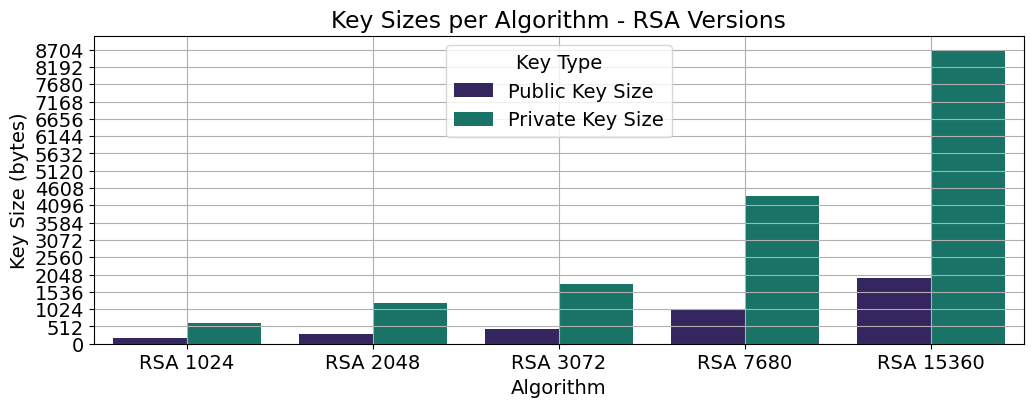
\includegraphics[width=1\textwidth]{Immagini/20240822_i9/Key_Sizes/KC_rsa.png}
    \caption{Dimensione delle chiavi private e pubbliche di RSA in funzione dei \textit{Modulus}}
    \label{fig:KC_rsa}
\end{figure}

\begin{figure}[H]
    \centering
    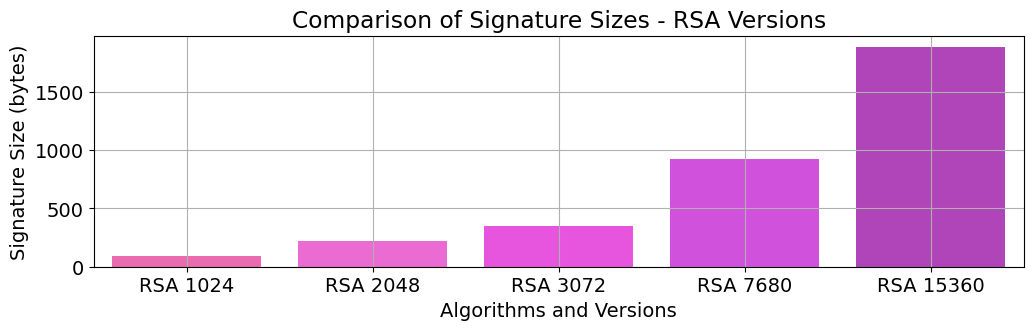
\includegraphics[width=1\textwidth]{Immagini/20240822_i9/Message_IO/IO_rsa.png}
    \caption{Dimensione delle firme di RSA in funzione dei \textit{Modulus}}
    \label{fig:IO_rsa}
\end{figure}

Per quanto riguarda la dimensione delle chiavi, entrambe contengono il \textit{Modulus} tuttavia:
\begin{enumerate}
    \item la chiave pubblica contiene pochi altri dati, per cui la sua dimensione finale (in Bytes) è poco maggiore a quella del \textit{Modulus} (espresso in bits).
    \item la chiave privata contiene molti altri parametri, per cui genericamente possiede una dimensione circa 4 volte maggiore rispetto al \textit{Modulus} (espresso in bits) \cite{stackexchange_rsa_2015}.
\end{enumerate}

Nei grafici \ref{fig:KC_rsa} e \ref{fig:IO_rsa} le dimensioni delle chiavi e delle firme crescono vertiginosamente all'aumentare della dimensione del \textit{Modulus}. Considerando il caso in cui il \textit{Modulus} è pari a 15360 bits, vuol dire che esso rappresenta un numero intero positivo dal valore compreso tra \( 2^{15359} \) e \(2^{15360} \), valore non rappresentabile da nessun tipo di hardware tradizionale. Per tale motivo è ragionevole che i tempi di generazione delle chiavi siano così elevati.

Al di là delle vulnerabilità di sicurezza che lo coinvolgono, è difficile immaginare un ampio utilizzo di RSA nei prossimi decenni se l'aumento del livello di sicurezza introduce calcoli così complessi da rendere i tempi di esecuzione proibitivi.

\begin{figure}[H]
    \centering
    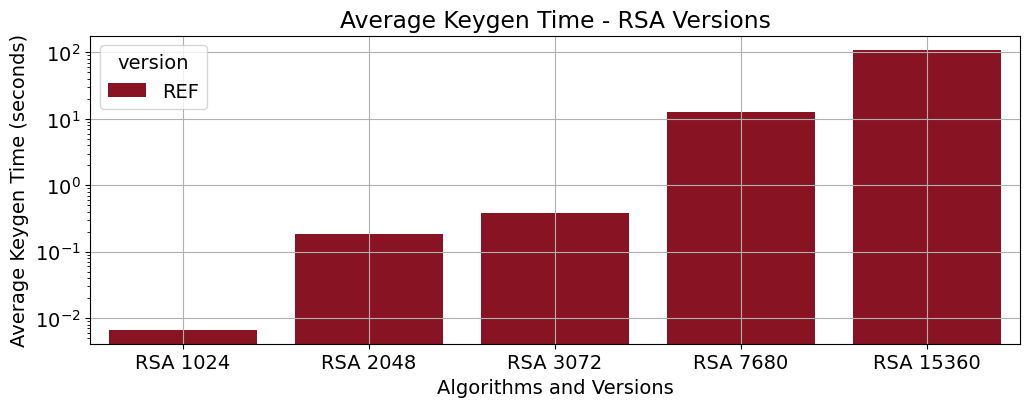
\includegraphics[width=1\textwidth]{Immagini/20240822_i9/Time_Keygen/TM_KG_rsa.png}
    \caption{Tempo di generazione delle chiavi di RSA in funzione dei \textit{Modulus}. Tempi misurati su PC\#1}.
    \label{fig:TM_KG_rsa}
\end{figure}

Il grafico \ref{fig:TM_KG_rsa} dimostra che anche i tempi di generazione della chiavi esplodono in maniera esponenziale, richiedendo decine di secondi per le versioni di RSA più sicure (misurati sull'hardware PC\#1).

\begin{figure}[H]
    \centering
    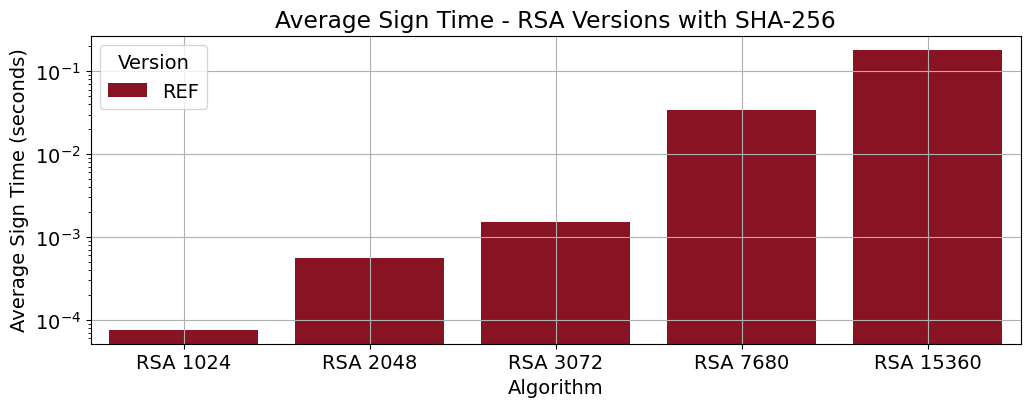
\includegraphics[width=1\textwidth]{Immagini/20240822_i9/Time_Sign/TM_SG_H_rsa_sha256.png}
    \caption{Tempi di firma di RSA eseguito su messaggi di lunghezza fissa 32 byte}
    \label{fig:TM_SG_H_rsa_sha256}
\end{figure}

\begin{figure}[H]
    \centering
    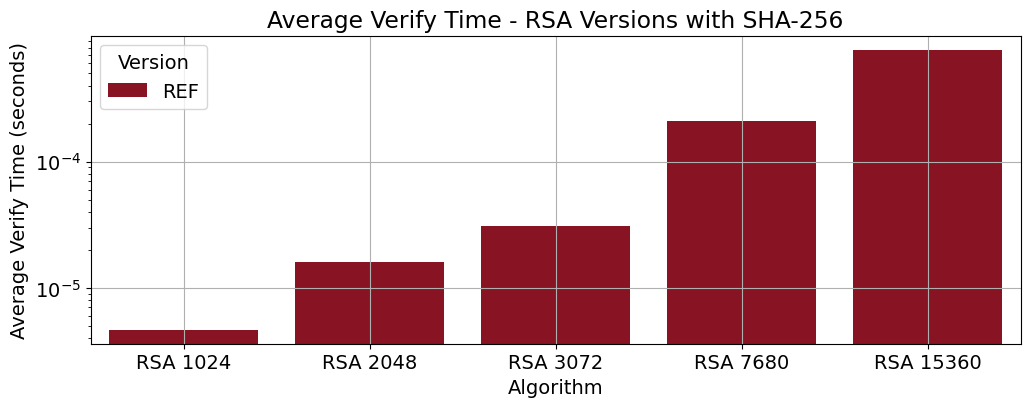
\includegraphics[width=1\textwidth]{Immagini/20240822_i9/Time_Verify/TM_VF_H_rsa_sha256.png}
    \caption{Tempi di verifica di RSA eseguito su messaggi di lunghezza fissa 32 byte}
    \label{fig:TM_VF_H_rsa_sha256}
\end{figure}

Allo stesso modo nei grafici \ref{fig:TM_SG_H_rsa_sha256} e \ref{fig:TM_VF_H_rsa_sha256} si notano gli stessi comportamenti nel caso di firma di un messaggio (che ha subito una fase di \textit{hashing} con \textit{SHA-256}) e nel caso di verifica della firma di un messaggio. I tempi aumentano esponenzialmente ma rimangono accettabili per eseguire più firme e verifiche in un breve tempo.

\begin{table}[H]
    \centering
    \begin{tabular}{lccccc}
        \toprule
        \textbf{RSA con Modulus:} & \textbf{1024} & \textbf{2048} & \textbf{3072} & \textbf{7680} & \textbf{15360} \\
        \cmidrule(lr){1-6}
        \textbf{Dimensione chiave privata (bytes)} & 610 & 1193 & 1767 & 4364 & 8684 \\
        \textbf{Dimensione chiave pubblica (bytes)} & 162 & 294 & 422 & 998 & 1958 \\
        \textbf{Dimensione firma (bytes)} & 96 & 224 & 352 & 928 & 1856 \\
        \textbf{Livello di sicurezza} & 1 & 2 & 3 & 4 & 5 \\
        \textbf{Modulus (bits)} & 1024 & 2048 & 3072 & 7680 & 15360 \\
        \textbf{Tempo medio Key Gen (ms)} & 6.7 & 186.2 & 377.5 & 12749.6 & 109706.9 \\
        \textbf{Tempo medio firma SHA256 (ns)} & 71 & 531 & 1451 & 35299 & 181973 \\
        \textbf{Tempo medio firma SHA512 (ns)} & 81 & 545 & 1595 & 36041 & 182464 \\
        \textbf{Tempo medio verifica SHA256 (ns)} & 4.7 & 15 & 30 & 209 & 766 \\
        \textbf{Tempo medio verifica SHA512 (ns)} & 5.1 & 18 & 39 & 201 & 768 \\
        \bottomrule
    \end{tabular}
    \caption{Confronto tra diverse configurazioni di RSA. Tempi riferiti all'esecuzione su PC\#1}
    \label{tab:rsa_comparison}
\end{table}



\section{Confronti tra algoritmi}

Quest'ultima sezione ha l'obiettivo di confrontare direttamente gli algoritmi tra loro, al fine di evidenziare aspetti non rilevabili analizzando i candidati singolarmente. Per aggiungere un ulteriore metro di paragone sarà presente anche RSA (ove significativo).

Ciascun algoritmo verrà confrontato con gli altri candidati in funzione dei livelli di sicurezza. I grafici infatti conterranno solo versioni di algoritmi con livello di sicurezza pari o similare. Nelle colonne della tabella \ref{tab:securitylevels_summary} sono evidenziati i confronti eseguiti.
\begin{table}[H]
    \centering
    \begin{tabular}{lccccc}
        \toprule
        \textbf{Livello di sicurezza} & \textbf{Livello  1/2} & \textbf{Livello 3 } & \textbf{Livello 5} \\
        \cmidrule(lr){1-4}
        \textbf{CRYSTALS Dilithium} & Dilithium 2 & Dilithium 3 & Dilithium 5 \\
        \textbf{FALCON} & Falcon 512 & - & Falcon 1024 \\
        \textbf{SPHINCS+} & SPHINCS+ 128 & SPHINCS+ 192 & SPHINCS+ 256 \\
        \textbf{RSA} & RSA 2048 & RSA 3072 & RSA 15360 \\
        \bottomrule
    \end{tabular}
    \caption{Ogni colonna contiene gli algoritmi che hanno un livello di sicurezza confrontabile}
    \label{tab:securitylevels_summary}
\end{table}


\begin{figure}[H]
    \centering
    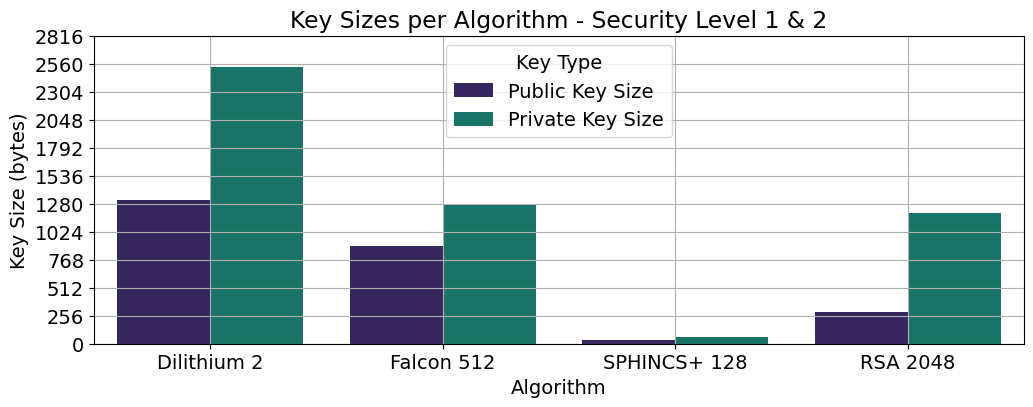
\includegraphics[width=1\textwidth]{Immagini/20240822_i9/Key_Sizes/KC_128bit_security_level.png}
    \caption{Dimensione delle chiavi private e pubbliche per gli algoritmi che offrono livello di sicurezza 1 o 2: CRYSTALS Dilithium, FALCON, SPHINCS+ e RSA}
    \label{fig:KC_128bit_security_level}
\end{figure}

\begin{figure}[H]
    \centering
    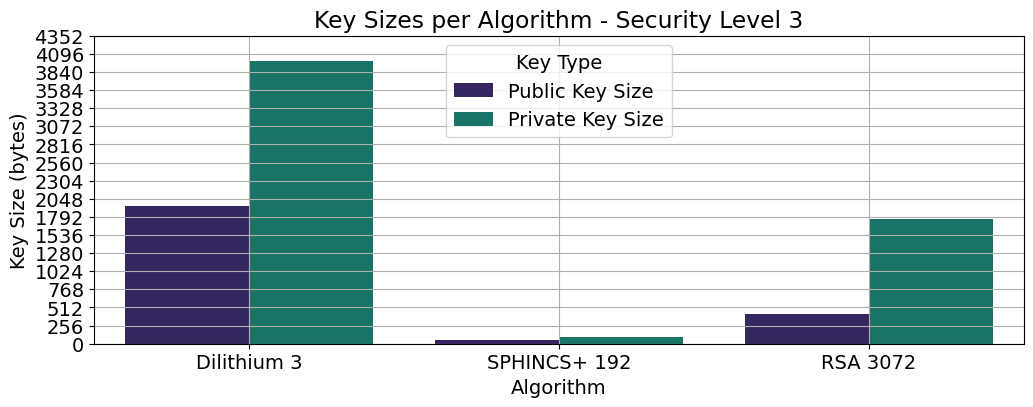
\includegraphics[width=1\textwidth]{Immagini/20240822_i9/Key_Sizes/KC_192bit_security_level.png}
    \caption{Dimensione delle chiavi private e pubbliche per gli algoritmi che offrono livello di sicurezza 3: CRYSTALS Dilithium, SPHINCS+ e RSA}
    \label{fig:KC_192bit_security_level}
\end{figure}

\begin{figure}[H]
    \centering
    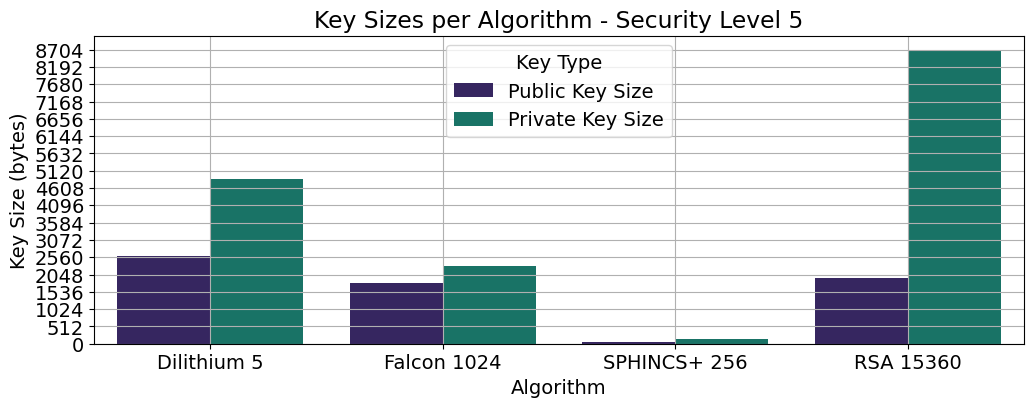
\includegraphics[width=1\textwidth]{Immagini/20240822_i9/Key_Sizes/KC_256bit_security_level.png}
    \caption{Dimensione delle chiavi private e pubbliche per gli algoritmi che offrono livello di sicurezza 5: CRYSTALS Dilithium, FALCON, SPHINCS+ e RSA}
    \label{fig:KC_256bit_security_level}
\end{figure}

I tre grafici precedenti (\ref{fig:KC_128bit_security_level} \ref{fig:KC_192bit_security_level} \ref{fig:KC_256bit_security_level}) si concentrano sul confrontare le dimensione delle chiavi, ciascuno a parità del livello di sicurezza trattato.

Uno degli aspetti non misurati direttamente ma che è possibile dedurre da questi grafici è la minimizzazione dei tempi di trasmissione: per minimizzare la trasmissione, a parità di bitrate, è necessario inviare un numero inferiore di pacchetti ethernet, la cui dimensione è di circa 1500 bytes. 

Le chiavi pubbliche sono spesso inviate assieme ai messaggi firmati, quindi sono contenute nelle comunicazioni. Tra i sistemi di firma digitale presenti nei grafici, gli unici che hanno la possibilità di mantenere una dimensione delle chiave pubblica limitata (tale da non richiedere più di un pacchetto) sono SPHINCS+, RSA e FALCON.

Per SPHINCS+ questo risultato è dettato dalla natura dell'algoritmo (\textit{Hash Based}) mentre per FALCON è un risultato degno di nota. Raramente gli algoritmi \textit{Lattice Based} riescono a ridurre le dimensioni delle chiavi in tal modo.

Un'altra cosa che si può comprendere è che RSA è completamente fuori scala se consideriamo la dimensione della chiave privata nella sua implementazione più sicura: questo rende le nuove proposte PQC un'ottima soluzione da standardizzare.

\begin{figure}[H]
    \centering
    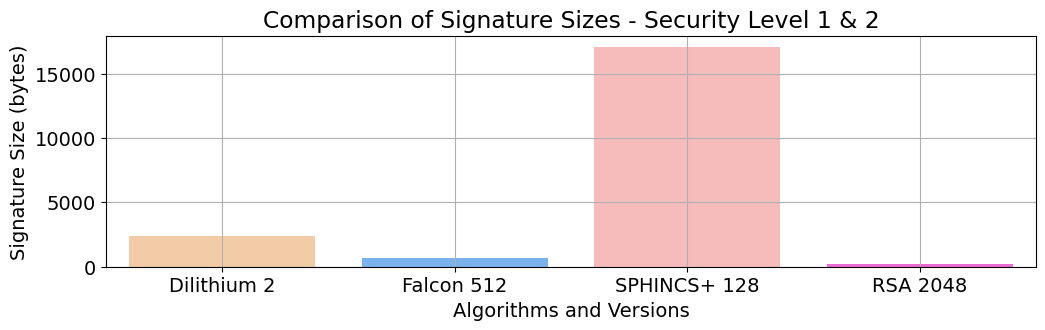
\includegraphics[width=1\textwidth]{Immagini/20240822_i9/Message_IO/IO_128bit_security_level.png}
    \caption{Dimensione della firma per gli algoritmi che offrono livello di sicurezza 1 e 2: CRYSTALS Dilithium, FALCON, SPHINCS+ e RSA}
    \label{fig:IO_128bit_security_level}
\end{figure}

\begin{figure}[H]
    \centering
    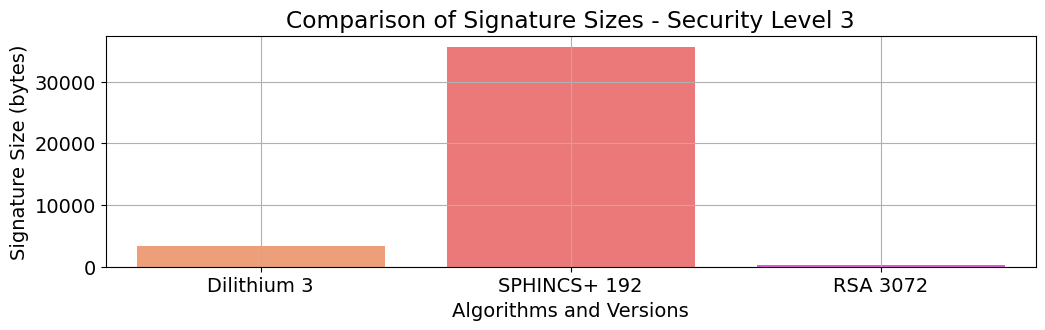
\includegraphics[width=1\textwidth]{Immagini/20240822_i9/Message_IO/IO_192bit_security_level.png}
    \caption{Dimensione della firma per gli algoritmi che offrono livello di sicurezza 3: CRYSTALS Dilithium, SPHINCS+ e RSA}
    \label{fig:IO_192bit_security_level}
\end{figure}

\begin{figure}[H]
    \centering
    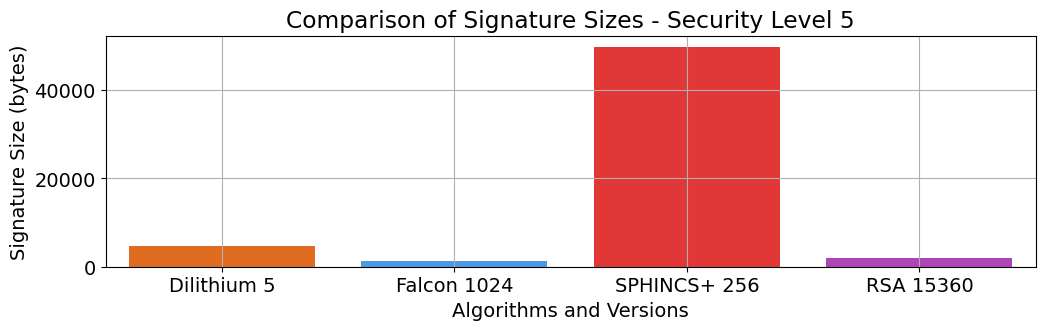
\includegraphics[width=1\textwidth]{Immagini/20240822_i9/Message_IO/IO_256bit_security_level.png}
    \caption{Dimensione della firma per gli algoritmi che offrono livello di sicurezza 5: CRYSTALS Dilithium, FALCON, SPHINCS+ e RSA}
    \label{fig:IO_256bit_security_level}
\end{figure}

Se consideriamo le dimensioni delle firme (trattate dai grafici \ref{fig:IO_128bit_security_level} \ref{fig:IO_192bit_security_level} \ref{fig:IO_256bit_security_level}) otteniamo altri aspetti di riflessione importanti: tra gli algoritmi PQC, FALCON sembra l'unico in grado di mantenere ridotta la trasmissione di una comunicazione firmata poiché è l'algoritmo che produce le firme di lunghezza inferiore.

L'obiettivo di \textit{compattezza} che il team di FALCON si è autoimposto ha molto valore se paragonato con le soluzioni attualmente in uso o candidate alla standardizzazione. SPHINCS+, sempre per la propria natura, produce delle firme di dimensioni significative, per cui richiederà grandi tempi di trasmissione rispetto agli altri algoritmi considerati.

\begin{figure}[H]
    \centering
    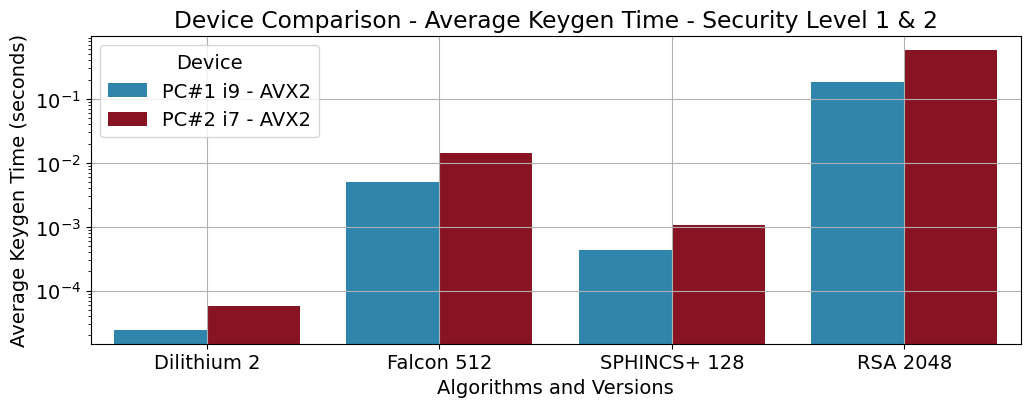
\includegraphics[width=1\textwidth]{Immagini/comparison/Time_Keygen/TM_KG_128bit_security_level.png}
    \caption{Tempi di generazione delle chiavi per gli algoritmi che offrono livello di sicurezza 1 e 2: CRYSTALS Dilithium, FALCON, SPHINCS+ e RSA}
    \label{fig:TM_KG_128bit_security_level}
\end{figure}

\begin{figure}[H]
    \centering
    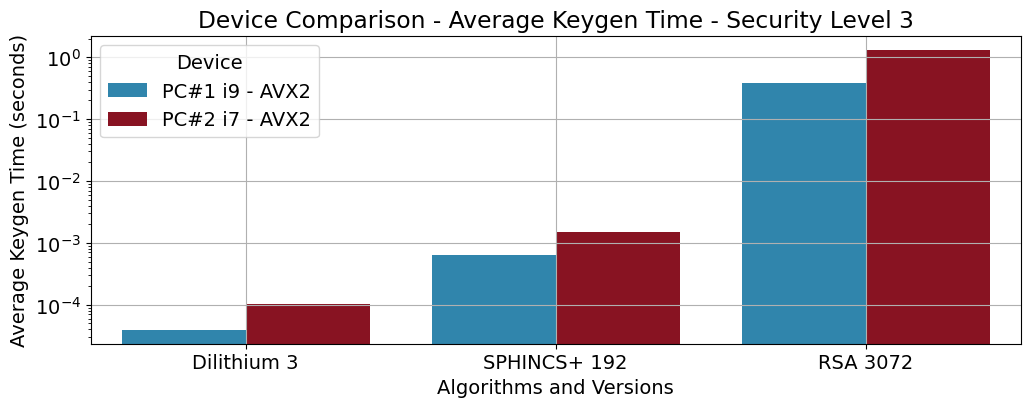
\includegraphics[width=1\textwidth]{Immagini/comparison/Time_Keygen/TM_KG_192bit_security_level.png}
    \caption{Tempi di generazione delle chiavi per gli algoritmi che offrono livello di sicurezza 3: CRYSTALS Dilithium, SPHINCS+ e RSA}
    \label{fig:TM_KG_192bit_security_level}
\end{figure}

\begin{figure}[H]
    \centering
    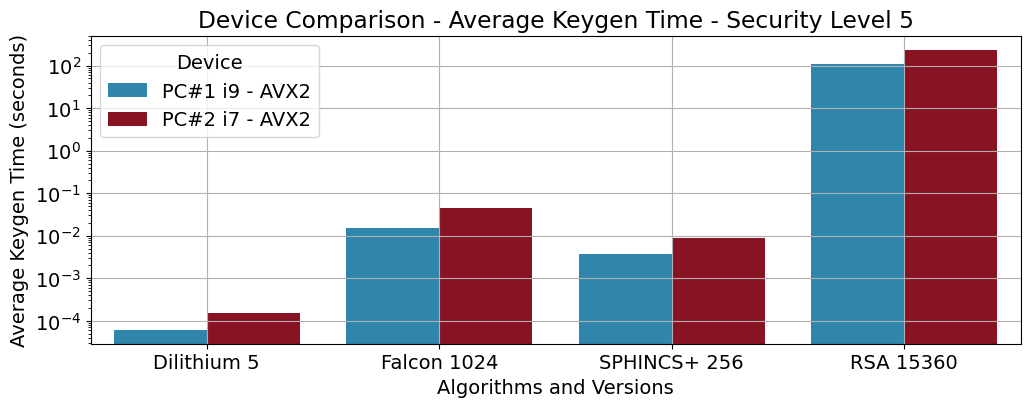
\includegraphics[width=1\textwidth]{Immagini/comparison/Time_Keygen/TM_KG_256bit_security_level.png}
    \caption{Tempi di generazione delle chiavi per gli algoritmi che offrono livello di sicurezza 5: CRYSTALS Dilithium, FALCON, SPHINCS+ e RSA}
    \label{fig:TM_KG_256bit_security_level}
\end{figure}

Per l'analisi dei tempi di generazione delle chiavi sono stati sviluppati i grafici \ref{fig:TM_KG_128bit_security_level} \ref{fig:TM_KG_192bit_security_level} \ref{fig:TM_KG_256bit_security_level}. Tra loro sono molto simili infatti, tra i vari livelli di sicurezza, si può notare che le differenze di prestazioni tra gli algoritmi sono mantenute in proporzione.

Come già anticipato, il NIST considera il tempo di generazioni chiavi come un aspetto secondario. Effettivamente questo ragionamento è intuitivo poiché questa procedura viene eseguita molte meno volte rispetto alle procedura di firma e verifica. In ogni caso, quando si parla di tempistiche, CRYSTALS Dilithium si mantiene tra i più veloci.

Per i tempi di firma e verifica verranno mostrati solo i grafici in cui i messaggi sono stati pre-elaborati con \textit{hashing} tramite \textit{SHA-256}. Ciò perché \textit{SHA-256} è attualmente il più utilizzato nelle firme \textit{AdES} (standard europeo presentato in introduzione) \cite{etsi_ts_119312}.
Indipendentemente dall'input, \textit{SHA-256} produrrà sempre una stringa di output la cui dimensione è 32 bytes, che verrà poi firmata.

\begin{figure}[H]
    \centering
    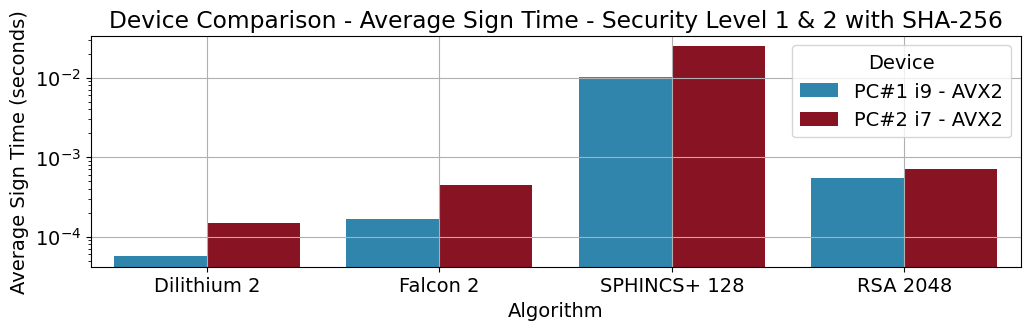
\includegraphics[width=1\textwidth]{Immagini/comparison/Time_Sign/TM_SG_H_128bit_security_level_sha256}
    \caption{Tempi di firma con messaggio di lunghezza fissa su PC\#1 e PC\#2 per gli algoritmi che offrono livello di sicurezza 1 e 2}
    \label{fig:TM_SG_H_128bit_security_level_sha256}
\end{figure}

\begin{figure}[H]
    \centering
    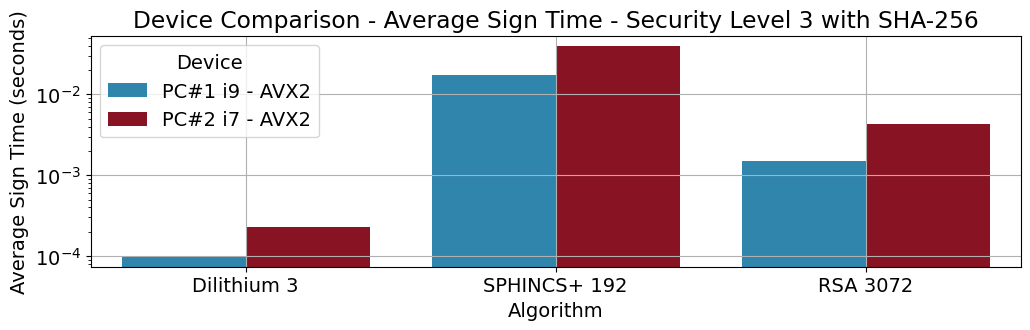
\includegraphics[width=1\textwidth]{Immagini/comparison/Time_Sign/TM_SG_H_192bit_security_level_sha256}
    \caption{Tempi di firma con messaggio di lunghezza fissa su PC\#1 e PC\#2 per gli algoritmi che offrono livello di sicurezza 3}
    \label{fig:TM_SG_H_192bit_security_level_sha256}
\end{figure}

\begin{figure}[H]
    \centering
    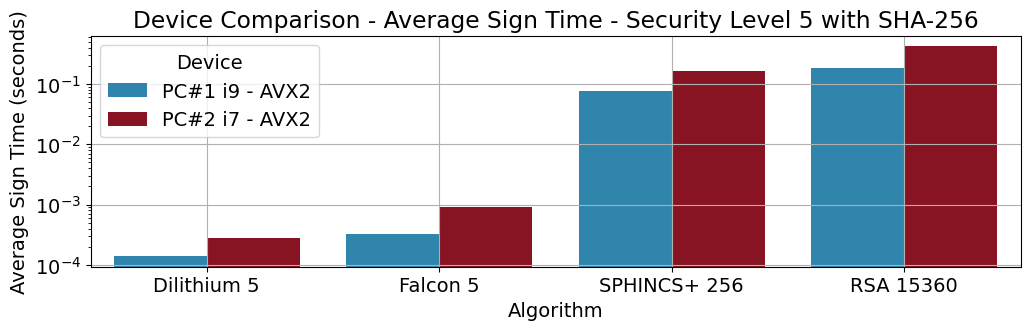
\includegraphics[width=1\textwidth]{Immagini/comparison/Time_Sign/TM_SG_H_256bit_security_level_sha256}
    \caption{Tempi di firma con messaggio di lunghezza fissa su PC\#1 e PC\#2 per gli algoritmi che offrono livello di sicurezza 5}
    \label{fig:TM_SG_H_256bit_security_level_sha256}
\end{figure}

\begin{figure}[H]
    \centering
    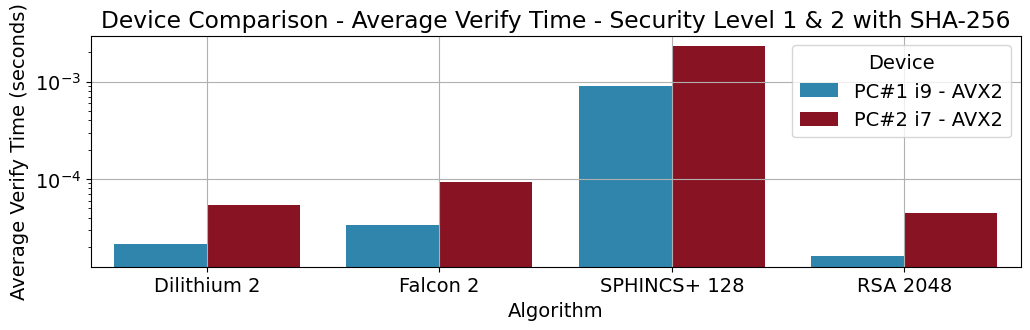
\includegraphics[width=1\textwidth]{Immagini/comparison/Time_Verify/TM_VF_H_128bit_security_level_sha256.png}
    \caption{Tempi di verifica con messaggio di lunghezza fissa su PC\#1 e PC\#2 per gli algoritmi che offrono livello di sicurezza 1 e 2}
    \label{fig:TM_VF_H_128bit_security_level_sha256}
\end{figure}

\begin{figure}[H]
    \centering
    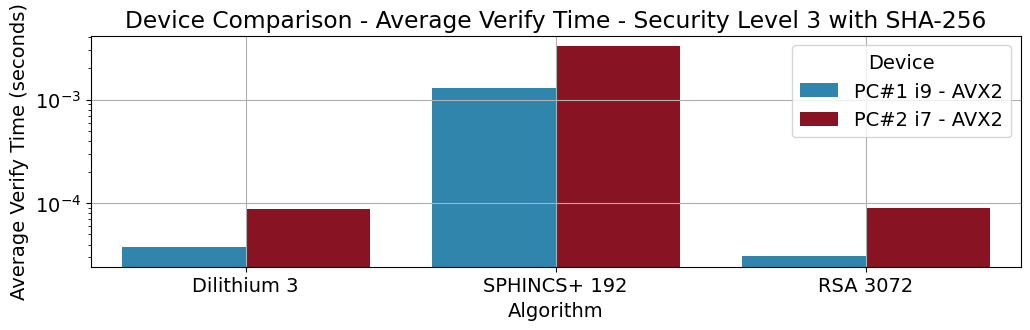
\includegraphics[width=1\textwidth]{Immagini/comparison/Time_Verify/TM_VF_H_192bit_security_level_sha256.png}
    \caption{Tempi di verifica con messaggio di lunghezza fissa su PC\#1 e PC\#2 per gli algoritmi che offrono livello di sicurezza 3}
    \label{fig:TM_VF_H_192bit_security_level_sha256}
\end{figure}

\begin{figure}[H]
    \centering
    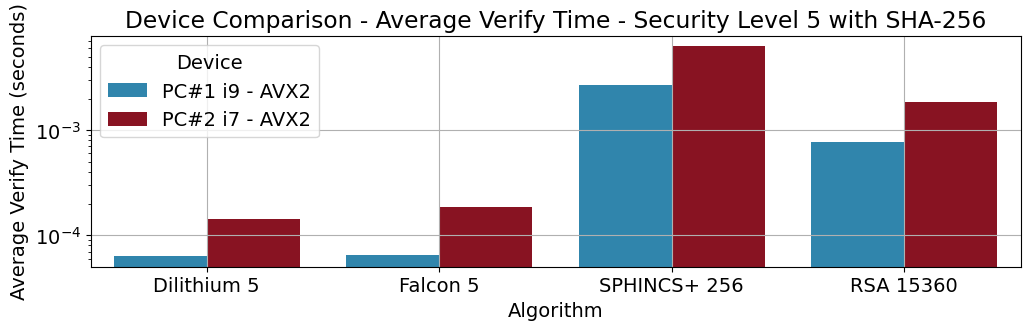
\includegraphics[width=1\textwidth]{Immagini/comparison/Time_Verify/TM_VF_H_256bit_security_level_sha256.png}
    \caption{Tempi di verifica con messaggio di lunghezza fissa su PC\#1 e PC\#2 per gli algoritmi che offrono livello di sicurezza 5}
    \label{fig:TM_VF_H_256bit_security_level_sha256}
\end{figure}

I grafici dei tempi di firma (\ref{fig:TM_SG_H_128bit_security_level_sha256}, \ref{fig:TM_SG_H_192bit_security_level_sha256}, \ref{fig:TM_SG_H_256bit_security_level_sha256}) e dei tempi di verifica (\ref{fig:TM_VF_H_128bit_security_level_sha256}, \ref{fig:TM_VF_H_192bit_security_level_sha256}, \ref{fig:TM_VF_H_256bit_security_level_sha256}) dimostrano che CRYSTALS Dilithium è il candidato con i tempi di firma minori e un'ottima soluzione anche nei tempi di verifica della firma.

CRYSTALS Dilithium ha delle prestazioni superiori (in termini di complessità temporale) a FALCON principalmente per due aspetti:
\begin{enumerate}
    \item FALCON include molte operazioni che coinvolgono numeri \textit{floating point}, per cui l'esecuzione in queste fasi risulta più onerosa.
    \item CRYSTALS Dilithium non riduce al minimo le dimensioni delle chiavi e delle firme, cosicché non ci siano fasi di compressione e espansione dei dati aggiuntive prima della vera e propria elaborazione.
\end{enumerate}

Ovviamente non c'è una scelta giusta o errata nelle implementazioni di FALCON e CRYSTALS Dilithium, tuttavia è interessante rilevare come le differenze concettuali e implementative si riflettano effettivamente nei risultati.

SPHINCS+ purtroppo è svantaggiato in questo tipo di competizioni: essendo un algoritmo \textit{Hash Based} le procedure di firma e verifica coinvolgono spesso fasi di \textit{hashing} che sono lente per loro natura. Per questo SPHINCS+, in tutte le sue versioni, risulta sempre almeno un ordine di grandezza più lento rispetto ai candidati appartenenti allo stesso livello di sicurezza.

Come per il confronto tra FALCON e CRYSTALS Dilithium, anche SPHINCS+ ha dei vantaggi: innanzitutto una forte dimostrazione teorica della sua sicurezza (poiché si basa su assunzioni matematiche \textit{semplici} rispetto ai \textit{Lattice Based}), alta compatibilità con diversi tipi di hardware e un utilizzo di memoria ridotto. Questo lo rende adatto ad essere eseguito nei dispositivi con processori ARM oppure nei dispositivi IoT (\textit{Internet of Things}) che mancano della compatibilità con le ottimizzazioni AVX2. Difatti SPHINCS+ possiede molte versioni rispetto agli altri candidati: ciascuna variante porta al suo interno tecniche diverse per eseguire gli stessi procedimenti oppure ottimizzazioni diverse.

La considerazione fondamentale che è possibile estrapolare dai precedenti grafici riguarda i tempi di esecuzione dei nuovi algoritmi PQC: essi sono conformi alla complessità temporale dei sistemi di firma digitale attualmente utilizzati. I tempi di RSA per le operazioni di firma e verifica sono pienamente compatibili con i tempi di questi candidati. Quest'ultimo aspetto dimostra ancora una volta che i candidati considerati sono maturi e pronti per la standardizzazione, come definito dal NIST nell'ultimo report \cite{NISTthirdReport}.